\documentclass{article}\usepackage[]{graphicx}\usepackage[]{color}
%% maxwidth is the original width if it is less than linewidth
%% otherwise use linewidth (to make sure the graphics do not exceed the margin)
\makeatletter
\def\maxwidth{ %
  \ifdim\Gin@nat@width>\linewidth
    \linewidth
  \else
    \Gin@nat@width
  \fi
}
\makeatother

\definecolor{fgcolor}{rgb}{0.345, 0.345, 0.345}
\newcommand{\hlnum}[1]{\textcolor[rgb]{0.686,0.059,0.569}{#1}}%
\newcommand{\hlstr}[1]{\textcolor[rgb]{0.192,0.494,0.8}{#1}}%
\newcommand{\hlcom}[1]{\textcolor[rgb]{0.678,0.584,0.686}{\textit{#1}}}%
\newcommand{\hlopt}[1]{\textcolor[rgb]{0,0,0}{#1}}%
\newcommand{\hlstd}[1]{\textcolor[rgb]{0.345,0.345,0.345}{#1}}%
\newcommand{\hlkwa}[1]{\textcolor[rgb]{0.161,0.373,0.58}{\textbf{#1}}}%
\newcommand{\hlkwb}[1]{\textcolor[rgb]{0.69,0.353,0.396}{#1}}%
\newcommand{\hlkwc}[1]{\textcolor[rgb]{0.333,0.667,0.333}{#1}}%
\newcommand{\hlkwd}[1]{\textcolor[rgb]{0.737,0.353,0.396}{\textbf{#1}}}%

\usepackage{framed}
\makeatletter
\newenvironment{kframe}{%
 \def\at@end@of@kframe{}%
 \ifinner\ifhmode%
  \def\at@end@of@kframe{\end{minipage}}%
  \begin{minipage}{\columnwidth}%
 \fi\fi%
 \def\FrameCommand##1{\hskip\@totalleftmargin \hskip-\fboxsep
 \colorbox{shadecolor}{##1}\hskip-\fboxsep
     % There is no \\@totalrightmargin, so:
     \hskip-\linewidth \hskip-\@totalleftmargin \hskip\columnwidth}%
 \MakeFramed {\advance\hsize-\width
   \@totalleftmargin\z@ \linewidth\hsize
   \@setminipage}}%
 {\par\unskip\endMakeFramed%
 \at@end@of@kframe}
\makeatother

\definecolor{shadecolor}{rgb}{.97, .97, .97}
\definecolor{messagecolor}{rgb}{0, 0, 0}
\definecolor{warningcolor}{rgb}{1, 0, 1}
\definecolor{errorcolor}{rgb}{1, 0, 0}
\newenvironment{knitrout}{}{} % an empty environment to be redefined in TeX

\usepackage{alltt}
\usepackage[vmargin=1in,hmargin=1in]{geometry}
\usepackage{enumerate}
\IfFileExists{upquote.sty}{\usepackage{upquote}}{}
\begin{document}
\title{Homework 3}
\date{BSAD 8700 - Business Analytics\\ Due: February 2, 2015}
\author{Kris Hanus, Laura Glathar, Arkya Rakshit, Jace Crist, Brandon Dlugosz\\ University of Nebraska at Omaha}
\maketitle

\textbf{ANSWER FOR 8:} \\


\begin{enumerate}[(a)]
\item
\begin{knitrout}
\definecolor{shadecolor}{rgb}{0.969, 0.969, 0.969}\color{fgcolor}\begin{kframe}
\begin{alltt}
\hlkwd{head}\hlstd{(Auto,}\hlnum{3}\hlstd{)}
\end{alltt}
\begin{verbatim}
##   mpg cylinders displacement horsepower weight acceleration year origin
## 1  18         8          307        130   3504         12.0   70      1
## 2  15         8          350        165   3693         11.5   70      1
## 3  18         8          318        150   3436         11.0   70      1
##                        name
## 1 chevrolet chevelle malibu
## 2         buick skylark 320
## 3        plymouth satellite
\end{verbatim}
\end{kframe}
\end{knitrout}
\begin{enumerate}[(i)]
\item
\begin{knitrout}
\definecolor{shadecolor}{rgb}{0.969, 0.969, 0.969}\color{fgcolor}\begin{kframe}
\begin{alltt}
\hlstd{predict1}\hlkwb{<-}\hlkwd{lm}\hlstd{(mpg}\hlopt{~}\hlstd{horsepower,} \hlkwc{data}\hlstd{=Auto)}
\hlkwd{summary}\hlstd{(predict1)}
\end{alltt}
\begin{verbatim}
## 
## Call:
## lm(formula = mpg ~ horsepower, data = Auto)
## 
## Residuals:
##      Min       1Q   Median       3Q      Max 
## -13.5710  -3.2592  -0.3435   2.7630  16.9240 
## 
## Coefficients:
##              Estimate Std. Error t value Pr(>|t|)    
## (Intercept) 39.935861   0.717499   55.66   <2e-16 ***
## horsepower  -0.157845   0.006446  -24.49   <2e-16 ***
## ---
## Signif. codes:  0 '***' 0.001 '**' 0.01 '*' 0.05 '.' 0.1 ' ' 1
## 
## Residual standard error: 4.906 on 390 degrees of freedom
## Multiple R-squared:  0.6059,	Adjusted R-squared:  0.6049 
## F-statistic: 599.7 on 1 and 390 DF,  p-value: < 2.2e-16
\end{verbatim}
\end{kframe}
\end{knitrout}
There is a very strong relationship between the predictor and the response variable. However, according to the hypothesis we would suggest that there might be a transformation that would allow us to create a better prediction. This can be seen from plotting that the Beta values may not be under the assumption of linearity.

\begin{knitrout}
\definecolor{shadecolor}{rgb}{0.969, 0.969, 0.969}\color{fgcolor}\begin{kframe}
\begin{alltt}
\hlkwd{ggplot}\hlstd{(Auto,} \hlkwd{aes}\hlstd{(horsepower, mpg))}\hlopt{+}\hlkwd{geom_point}\hlstd{()}
\end{alltt}
\end{kframe}
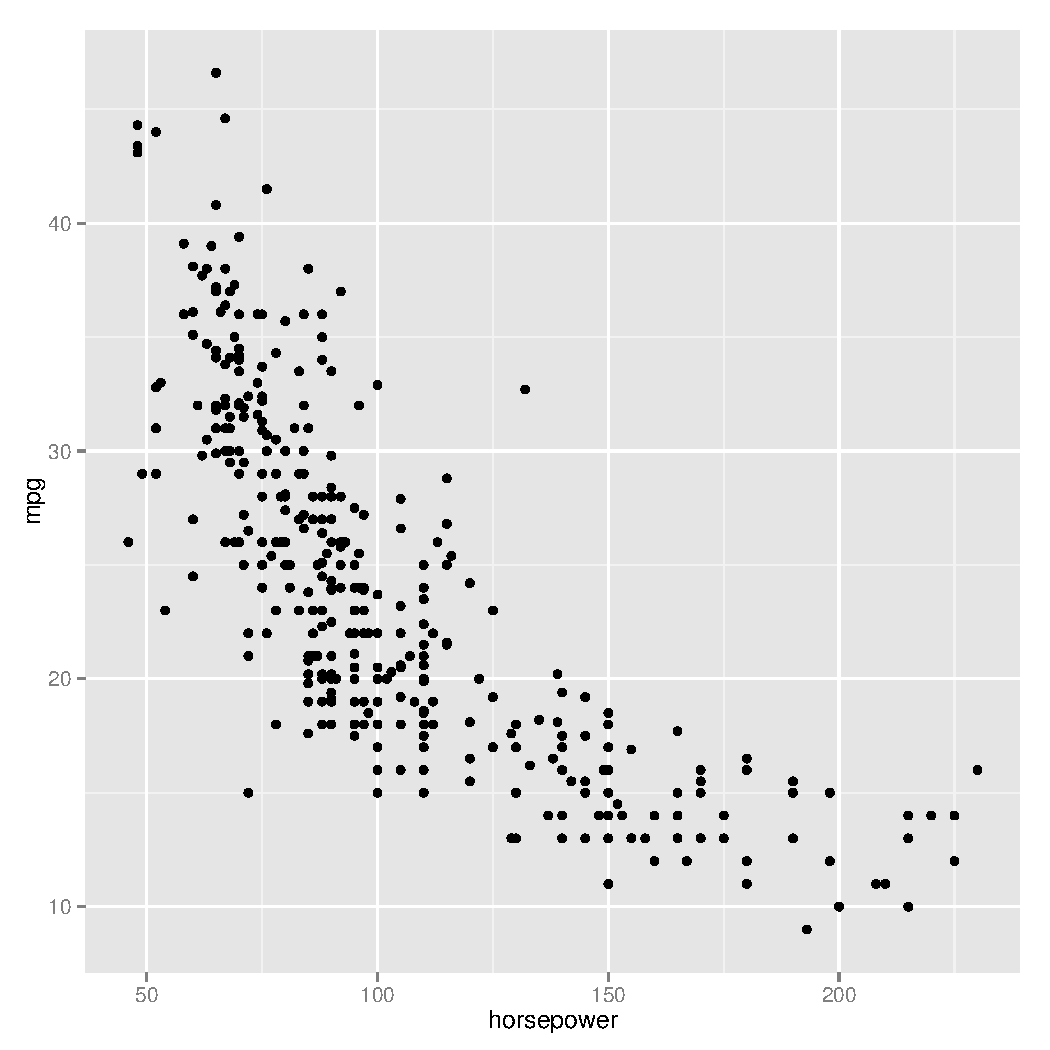
\includegraphics[width=\maxwidth]{figure/unnamed-chunk-4-1} 

\end{knitrout}

\item
\begin{knitrout}
\definecolor{shadecolor}{rgb}{0.969, 0.969, 0.969}\color{fgcolor}\begin{kframe}
\begin{alltt}
\hlstd{fvalue}\hlkwb{<-}\hlkwd{qf}\hlstd{(}\hlnum{.95}\hlstd{,}\hlnum{390}\hlstd{,}\hlnum{1}\hlstd{)}
\hlstd{fvalue}
\end{alltt}
\begin{verbatim}
## [1] 253.9873
\end{verbatim}
\end{kframe}
\end{knitrout}
The Adjusted R-Squared value would suggest that a linear line would fit the data fairly well, but as the F-statistic shows and p-value supports that the fit is significant. However, as can be shown by graph or residuals this is a curvi-linear plot. We would need either a transformation or an adjusted curvi-linear independent value.

\item

\begin{knitrout}
\definecolor{shadecolor}{rgb}{0.969, 0.969, 0.969}\color{fgcolor}\begin{kframe}
\begin{alltt}
\hlkwd{cor}\hlstd{(Auto[}\hlnum{1}\hlopt{:}\hlnum{8}\hlstd{])}
\end{alltt}
\begin{verbatim}
##                     mpg  cylinders displacement horsepower     weight
## mpg           1.0000000 -0.7776175   -0.8051269 -0.7784268 -0.8322442
## cylinders    -0.7776175  1.0000000    0.9508233  0.8429834  0.8975273
## displacement -0.8051269  0.9508233    1.0000000  0.8972570  0.9329944
## horsepower   -0.7784268  0.8429834    0.8972570  1.0000000  0.8645377
## weight       -0.8322442  0.8975273    0.9329944  0.8645377  1.0000000
## acceleration  0.4233285 -0.5046834   -0.5438005 -0.6891955 -0.4168392
## year          0.5805410 -0.3456474   -0.3698552 -0.4163615 -0.3091199
## origin        0.5652088 -0.5689316   -0.6145351 -0.4551715 -0.5850054
##              acceleration       year     origin
## mpg             0.4233285  0.5805410  0.5652088
## cylinders      -0.5046834 -0.3456474 -0.5689316
## displacement   -0.5438005 -0.3698552 -0.6145351
## horsepower     -0.6891955 -0.4163615 -0.4551715
## weight         -0.4168392 -0.3091199 -0.5850054
## acceleration    1.0000000  0.2903161  0.2127458
## year            0.2903161  1.0000000  0.1815277
## origin          0.2127458  0.1815277  1.0000000
\end{verbatim}
\end{kframe}
\end{knitrout}
There is a negative relationship

\item
\begin{knitrout}
\definecolor{shadecolor}{rgb}{0.969, 0.969, 0.969}\color{fgcolor}\begin{kframe}
\begin{alltt}
\hlstd{NewDat}\hlkwb{<-}\hlkwd{data.frame}\hlstd{(}\hlkwc{horsepower}\hlstd{=}\hlnum{98}\hlstd{)}
\hlkwd{predict}\hlstd{(predict1, NewDat,}\hlkwc{interval} \hlstd{=} \hlstr{"confidence"}\hlstd{,} \hlkwc{level}\hlstd{=}\hlnum{0.95}\hlstd{,} \hlkwc{se.fit}\hlstd{=}\hlnum{FALSE}\hlstd{)}
\end{alltt}
\begin{verbatim}
##        fit      lwr      upr
## 1 24.46708 23.97308 24.96108
\end{verbatim}
\begin{alltt}
\hlkwd{predict}\hlstd{(predict1, NewDat,}\hlkwc{interval} \hlstd{=} \hlstr{"prediction"}\hlstd{,} \hlkwc{level}\hlstd{=}\hlnum{0.95}\hlstd{,} \hlkwc{se.fit}\hlstd{=}\hlnum{FALSE}\hlstd{)}
\end{alltt}
\begin{verbatim}
##        fit     lwr      upr
## 1 24.46708 14.8094 34.12476
\end{verbatim}
\end{kframe}
\end{knitrout}
\end{enumerate}
\item
\begin{knitrout}
\definecolor{shadecolor}{rgb}{0.969, 0.969, 0.969}\color{fgcolor}\begin{kframe}
\begin{alltt}
\hlkwd{ggplot}\hlstd{(Auto,} \hlkwd{aes}\hlstd{(horsepower,mpg))}\hlopt{+}
  \hlkwd{geom_point}\hlstd{()}\hlopt{+}
  \hlkwd{geom_abline}\hlstd{(}\hlkwc{intercept}\hlstd{=}\hlnum{39.93}\hlstd{,} \hlkwc{slope}\hlstd{=}\hlopt{-}\hlnum{0.157845}\hlstd{)}
\end{alltt}
\end{kframe}
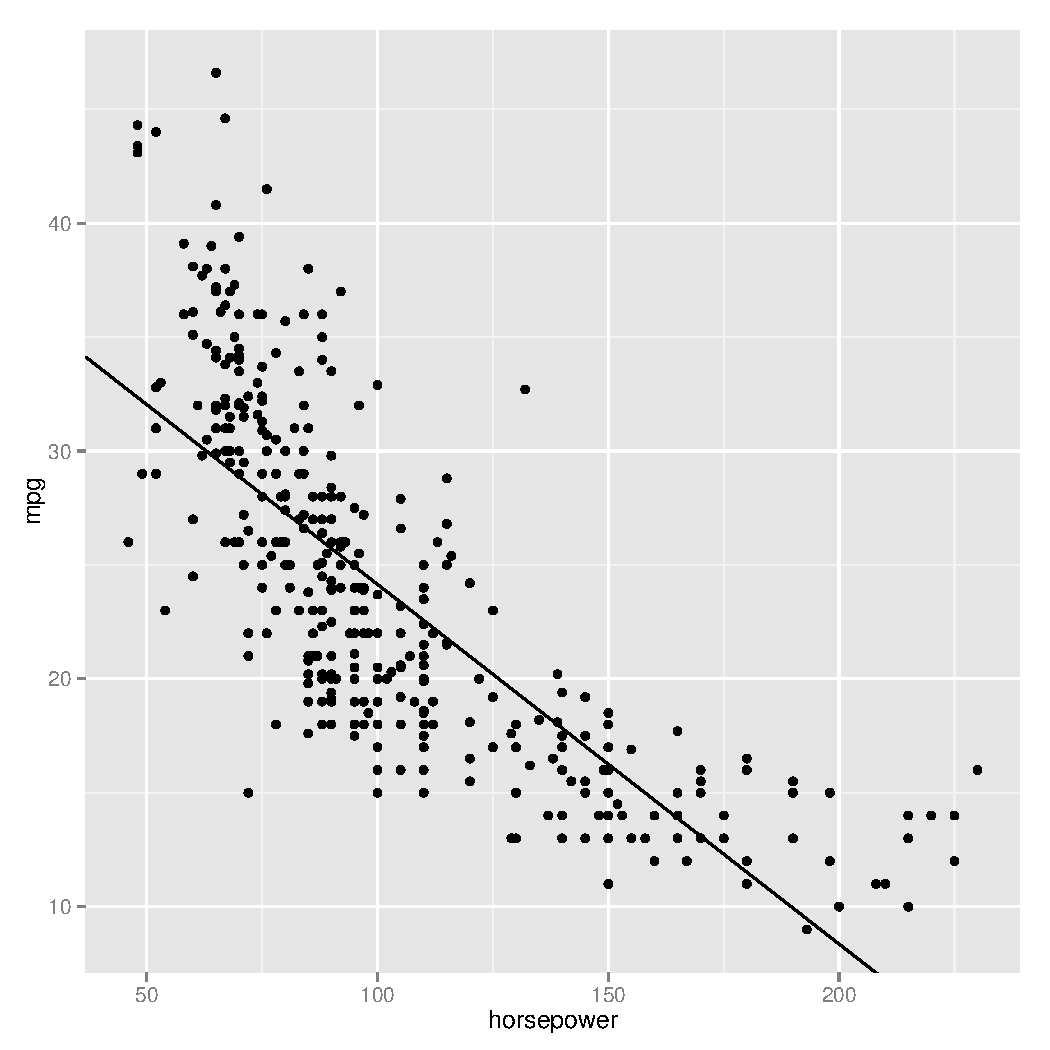
\includegraphics[width=\maxwidth]{figure/unnamed-chunk-8-1} 

\end{knitrout}

\item
Extra Credit:
\begin{knitrout}
\definecolor{shadecolor}{rgb}{0.969, 0.969, 0.969}\color{fgcolor}\begin{kframe}
\begin{alltt}
\hlkwd{ggplot}\hlstd{(Auto,} \hlkwd{aes}\hlstd{(horsepower,mpg))}\hlopt{+}\hlkwd{geom_point}\hlstd{()}\hlopt{+}
  \hlkwd{geom_abline}\hlstd{(}\hlkwc{intercept}\hlstd{=}\hlnum{39.93}\hlstd{,} \hlkwc{slope}\hlstd{=}\hlopt{-}\hlnum{0.157845}\hlstd{)}\hlopt{+}
  \hlkwd{geom_smooth}\hlstd{(}\hlkwc{method}\hlstd{=}\hlstr{"lm"}\hlstd{,} \hlkwc{se}\hlstd{=T)}
\end{alltt}
\end{kframe}
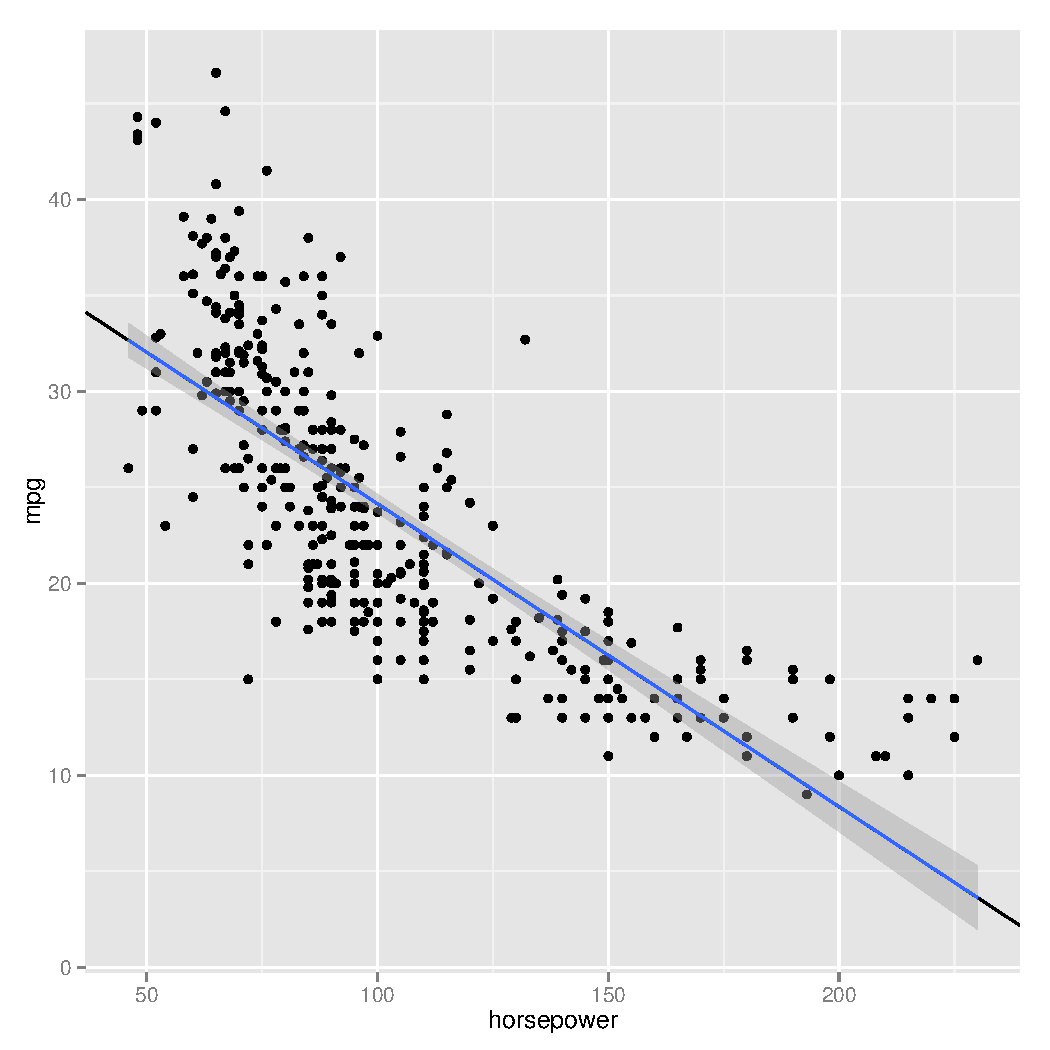
\includegraphics[width=\maxwidth]{figure/unnamed-chunk-9-1} 

\end{knitrout}
The fitted line goes through the mean. It is evident that the residuals of the points (from left to right) would start off positive, would then become negative, and will finish positive. By looking at this trend we would suggest that the data is either logistic or $\frac{1}{x}$ and there might be a better fit model to the data.
\end{enumerate}

\textbf{ANSWER FOR 9:} \\
\begin{enumerate}[(a)]

\item
\begin{knitrout}
\definecolor{shadecolor}{rgb}{0.969, 0.969, 0.969}\color{fgcolor}\begin{kframe}
\begin{alltt}
\hlkwd{pairs}\hlstd{(Auto)}
\end{alltt}
\end{kframe}
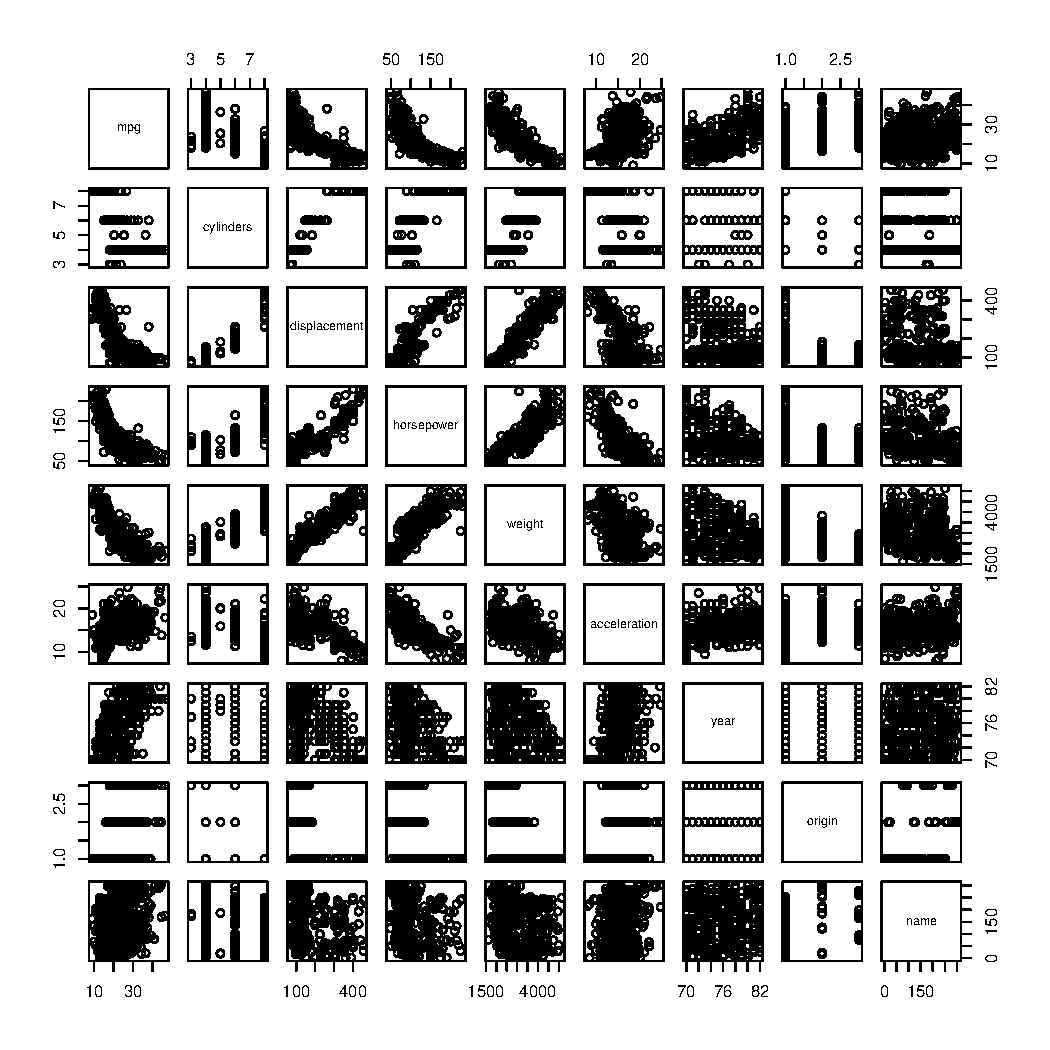
\includegraphics[width=\maxwidth]{figure/unnamed-chunk-10-1} 

\end{knitrout}

\item
\begin{knitrout}
\definecolor{shadecolor}{rgb}{0.969, 0.969, 0.969}\color{fgcolor}\begin{kframe}
\begin{alltt}
\hlkwd{str}\hlstd{(Auto)}
\end{alltt}
\begin{verbatim}
## 'data.frame':	392 obs. of  9 variables:
##  $ mpg         : num  18 15 18 16 17 15 14 14 14 15 ...
##  $ cylinders   : num  8 8 8 8 8 8 8 8 8 8 ...
##  $ displacement: num  307 350 318 304 302 429 454 440 455 390 ...
##  $ horsepower  : num  130 165 150 150 140 198 220 215 225 190 ...
##  $ weight      : num  3504 3693 3436 3433 3449 ...
##  $ acceleration: num  12 11.5 11 12 10.5 10 9 8.5 10 8.5 ...
##  $ year        : num  70 70 70 70 70 70 70 70 70 70 ...
##  $ origin      : num  1 1 1 1 1 1 1 1 1 1 ...
##  $ name        : Factor w/ 304 levels "amc ambassador brougham",..: 49 36 231 14 161 141 54 223 241 2 ...
\end{verbatim}
\begin{alltt}
\hlkwd{cor}\hlstd{(Auto[}\hlnum{1}\hlopt{:}\hlnum{8}\hlstd{])}
\end{alltt}
\begin{verbatim}
##                     mpg  cylinders displacement horsepower     weight
## mpg           1.0000000 -0.7776175   -0.8051269 -0.7784268 -0.8322442
## cylinders    -0.7776175  1.0000000    0.9508233  0.8429834  0.8975273
## displacement -0.8051269  0.9508233    1.0000000  0.8972570  0.9329944
## horsepower   -0.7784268  0.8429834    0.8972570  1.0000000  0.8645377
## weight       -0.8322442  0.8975273    0.9329944  0.8645377  1.0000000
## acceleration  0.4233285 -0.5046834   -0.5438005 -0.6891955 -0.4168392
## year          0.5805410 -0.3456474   -0.3698552 -0.4163615 -0.3091199
## origin        0.5652088 -0.5689316   -0.6145351 -0.4551715 -0.5850054
##              acceleration       year     origin
## mpg             0.4233285  0.5805410  0.5652088
## cylinders      -0.5046834 -0.3456474 -0.5689316
## displacement   -0.5438005 -0.3698552 -0.6145351
## horsepower     -0.6891955 -0.4163615 -0.4551715
## weight         -0.4168392 -0.3091199 -0.5850054
## acceleration    1.0000000  0.2903161  0.2127458
## year            0.2903161  1.0000000  0.1815277
## origin          0.2127458  0.1815277  1.0000000
\end{verbatim}
\end{kframe}
\end{knitrout}

\item
\begin{enumerate}[(i)]
\item
\begin{knitrout}
\definecolor{shadecolor}{rgb}{0.969, 0.969, 0.969}\color{fgcolor}\begin{kframe}
\begin{alltt}
\hlstd{lm.fit}\hlkwb{<-}\hlkwd{lm}\hlstd{(mpg}\hlopt{~}\hlstd{.,}\hlkwc{data}\hlstd{=Auto[}\hlnum{1}\hlopt{:}\hlnum{8}\hlstd{])}
\hlkwd{summary}\hlstd{(lm.fit)}
\end{alltt}
\begin{verbatim}
## 
## Call:
## lm(formula = mpg ~ ., data = Auto[1:8])
## 
## Residuals:
##     Min      1Q  Median      3Q     Max 
## -9.5903 -2.1565 -0.1169  1.8690 13.0604 
## 
## Coefficients:
##                Estimate Std. Error t value Pr(>|t|)    
## (Intercept)  -17.218435   4.644294  -3.707  0.00024 ***
## cylinders     -0.493376   0.323282  -1.526  0.12780    
## displacement   0.019896   0.007515   2.647  0.00844 ** 
## horsepower    -0.016951   0.013787  -1.230  0.21963    
## weight        -0.006474   0.000652  -9.929  < 2e-16 ***
## acceleration   0.080576   0.098845   0.815  0.41548    
## year           0.750773   0.050973  14.729  < 2e-16 ***
## origin         1.426141   0.278136   5.127 4.67e-07 ***
## ---
## Signif. codes:  0 '***' 0.001 '**' 0.01 '*' 0.05 '.' 0.1 ' ' 1
## 
## Residual standard error: 3.328 on 384 degrees of freedom
## Multiple R-squared:  0.8215,	Adjusted R-squared:  0.8182 
## F-statistic: 252.4 on 7 and 384 DF,  p-value: < 2.2e-16
\end{verbatim}
\begin{alltt}
\hlstd{lm.fit}\hlkwb{<-}\hlkwd{lm}\hlstd{(mpg}\hlopt{~}\hlstd{.}\hlopt{-}\hlstd{acceleration}\hlopt{-}\hlstd{cylinders}\hlopt{-}\hlstd{horsepower}\hlopt{-}\hlstd{displacement,}\hlkwc{data}\hlstd{=Auto[}\hlnum{1}\hlopt{:}\hlnum{8}\hlstd{])}
\hlkwd{summary}\hlstd{(lm.fit)}
\end{alltt}
\begin{verbatim}
## 
## Call:
## lm(formula = mpg ~ . - acceleration - cylinders - horsepower - 
##     displacement, data = Auto[1:8])
## 
## Residuals:
##     Min      1Q  Median      3Q     Max 
## -9.9440 -2.0948 -0.0389  1.7255 13.2722 
## 
## Coefficients:
##               Estimate Std. Error t value Pr(>|t|)    
## (Intercept) -1.805e+01  4.001e+00  -4.510 8.60e-06 ***
## weight      -5.994e-03  2.541e-04 -23.588  < 2e-16 ***
## year         7.571e-01  4.832e-02  15.668  < 2e-16 ***
## origin       1.150e+00  2.591e-01   4.439 1.18e-05 ***
## ---
## Signif. codes:  0 '***' 0.001 '**' 0.01 '*' 0.05 '.' 0.1 ' ' 1
## 
## Residual standard error: 3.348 on 388 degrees of freedom
## Multiple R-squared:  0.8175,	Adjusted R-squared:  0.816 
## F-statistic: 579.2 on 3 and 388 DF,  p-value: < 2.2e-16
\end{verbatim}
\end{kframe}
\end{knitrout}
There is some relationship between predictors and the response variable.
\item
 The variables which have the highest correlation would be weight, year, and origin. They are all significant to within $99.9\%$. There were two other variables (horsepower and displacement) that would have been significant together to a $90\%$, however; we are looking for correlations above $95\%$ and preventing over-fitting the model they were eliminated.
\item
The $\beta_{year}$ is equal to $.7571$. This is a positive correlation between year and mpg.
\end{enumerate}
\item
Extra Credit
\item
Extra Credit
\item
Extra Credit


\end{enumerate}
\end{document}
